\section{Program Validation and Verification}
\label{ss:progr-valid-verif}


WiFi mapper consists of two apps, and these are android app and web app. In order to examine the behaviour of the android app, it was tested on three devices. Upon installing the app, the users, moved around upper campus to collect data at different locations. This was done to test if the app was able to collect data from routers.

<<<<<<< HEAD
For each device that the app was installed, data points were saved on the database. The app also displayed the respective polygons on each WLAN zone across all the devices as the data was collected. This together with other functionalities proved that the app. To test the web app functionalities, the app was deployed and hosted on firebase.

Different devices were used to access the app and it displayed expected across all decices in a responsive manner.

=======
\begin{table}[h!]
  \centering
\caption{Summary Testing Plan. A table caption goes above the table.}
\begin{tabular}[t]{|p{8cm}|p{7cm}|} \hline
  \textbf{Process} & \textbf{Technique} \\ \hline 1. Class
    Testing: test methods and state behaviour of classes & Random,
    Partition and White-Box Tests \\ \hline 2. Integration Testing:
    test the
    interaction of sets of classes & Random and Behavioural Testing \\
    \hline 3. Validation Testing: test whether customer requirements
    are satisfied & Use-case based black box and Acceptance tests \\
    \hline 4. System Testing: test the behaviour of the system as part
    of a larger environment & Recovery, security, stress and
    performance tests \\ \hline
>>>>>>> dbdcaa9c489184e6c0f3ec2628a1dc42bc14dddc


Trello was used to create and manage a test plan for the WiFi mapper project. A board that consisted of items to be tested was created. Each item had a deadline attached to it.This board consisted of features that had been developed but were now waiting to be tested. Another board for items that were in the process of being tested so as to track the items  that were currently being tested. The last board that consisted of items on which testing had already been done was created.

To test each item different testing methodologies were used.

\subsection*{User Interface Testing}
To test the interaction of the user with the app, User Interface testing was used.This was done so as to test the user's interaction with the software. Different navigation functionalities on the map were tested and these involved zooming and panning on the map. Different users were given a running app, the behaviour of the app was noted as the users interacted with the software.User Interface testing ensures that the objects within the user interface function as expected and conform to required standards.

\subsection*{Database Testing}
Database models were tested so as to obtain proper database structure. Writing and querying of the database were also tested. For writing the app was tested for possible race conditions when the app is writing to the databse. For reading the queried data was compared with the expected output.

\subsection*{Unit testing}
To test all methods of objects unit testing was done. Unit testing ensured that all parts of the app are working as expected. To test static methods mock up for testing was used.

\subsection*{Volume Testing}
This kind of testing concerns testing the software for large amounts of data. This test was necessary for wifi mapper as the app keeps on collecting data on many different points. To perform this test multiple clients were used to collect data different points at the same time. As the app receive multiple data the its behaviour was noted.

\subsection*{Security and Access Control Testing}
Application security ensures that proper protection and integrity of data is ensured for all the users. WiFi mapper provides advanced user with private data. As a result the app did require such form of testing.

\subsection*{Failover and Recovery Testing}
Failover testing ensures that, for those systems that need to be kept running, when a failing condition occurs, then the alternate systems properly take over for the failed system without any severe loss of data or transactions. Being a near real-time app, wifi mapper needed to quickly from any failure events.

\begin{figure}
	\centering
	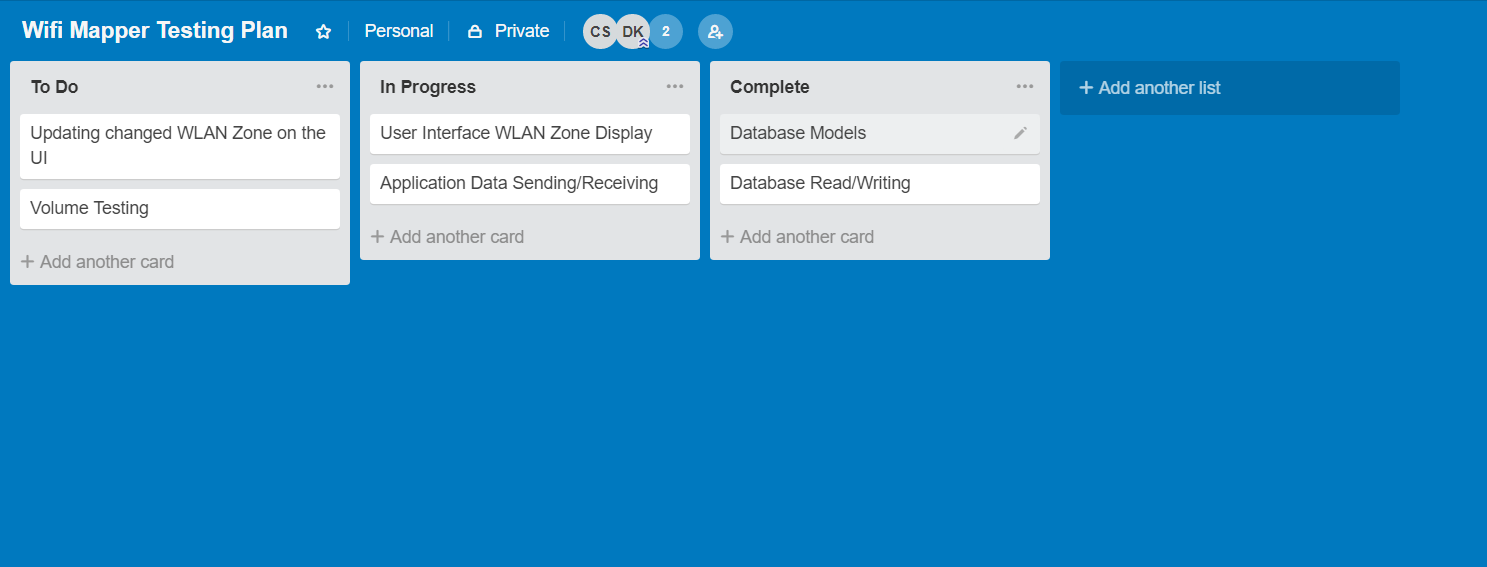
\includegraphics[width=0.7\linewidth]{images/testing_plan}
	\caption{Software management testing plan.}
	\label{fig:testingplan}
\end{figure}
\newpage

\begin{table}[h!]
  \centering
\caption{Summary Testing Plan.}

\begin{tabular}[t]{|p{8cm}|p{7cm}|} \hline

  \textbf{Process} & \textbf{Technique} \\ \hline 1. User Interface Testing: Test view navigation and features & Give user to interact with all the features \\ \hline 2.Database: Test database models and database read and write & Random read and write testing \\
    \hline 3.Volume testing: test application behaviour for large data sets & Random testing of the application with large datapoints \\
    \hline 4. Security and Access Control Testing: test how the application handles privacy & Recovery, security, stress and
    performance tests \\ \hline 5. Failover and Recovery Testing: testing how the application recovers from failure & Recovery, security, stress and
    performance tests  \\ \hline

\end{tabular}

\label{tab:test-plan}
\end{table}
